\chapter{Brute Force Approach}

In the previous chapter the correlation between the solar-zenith angle's cosine and the estimated VTEC value was studied. Here, we aim to provide a first, brute force approach, of the \textit{Blind GNSS Search of Extraterrestrial EUV Sources (BGSEES)} algorithm to estimate the location of a EUV source. This approach is done as a first approximation to be problem to see more clearly how the algorithm will work, regardless of the performance.

For this first approach the Sun is used as the source (to check the corectness of the solution). It considers possible Sun locations (with a certain degree of precision) and checks the fitness of each to consider which could be the real location.

\section{Key elements}

\subsection{Mean VTEC as a reliable indicator of the moment of the flare}

The first part of the algorithm was, without going into the actual computations regarding the position of the IPPs, the possible Sun locations, etc, finding out when to perform the study, that is, detecting a spike in the VTEC content throughout the provided data range. 
In the previous chapter we already knew the specific moment of the flare: 11.05h, and could work based on this information, but the first step of the algorithm has to determine which moment is going to be studied.

For each epoch\footnote{In our data set the epochs ranged from 10.5 to 11.5, that is, 10:30AM to 11:30AM with a sampling rate of 1/120 hours or 30 seconds} we computed the mean VTEC of all IPPs and returned the epoch which had the highest VTEC mean.

??????An alternative which performs an insertion sort (by inserting the epoch candidates into a priority queue) was also considered and implemented, but for this chapter we only used the epoch with the largest mean.

To see if the mean VTEC could be used as a reliable indicator, the algorithm was tested with all available epochs of the data set, in order to study the effect of this indicator in the resulting estimation of the source's location.

To do this we ordered the different epochs available in our data set by their mean VTEC, inserting them into a priority queue. \\

Figure \ref{fig:differentEpochs} shows the evolution of the correlation coefficient of the best estimated location (a) and its total error (right ascension error + declination error) (b) as the mean VTEC of the epoch decreases.

\clearpage

\begin{figure}[!htb]
	\begin{subfigure}[b]{0.5\textwidth}
		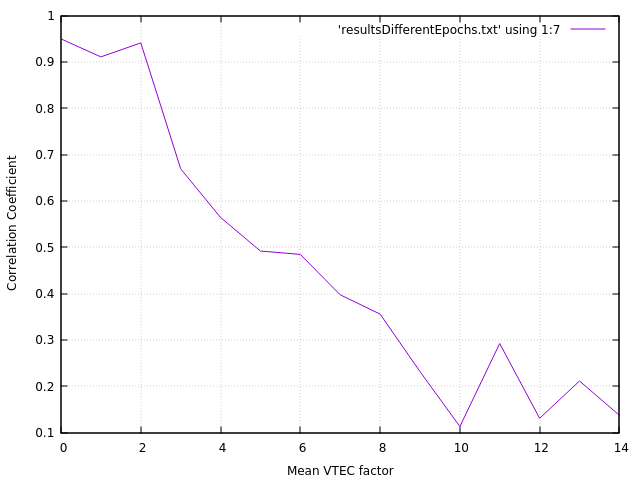
\includegraphics[width=\linewidth]{images/ch6/spikes/correlationDecrease.png}
		\caption{Correlation coefficient}
	\end{subfigure}
	\hfill
	\begin{subfigure}[b]{0.5\textwidth}
		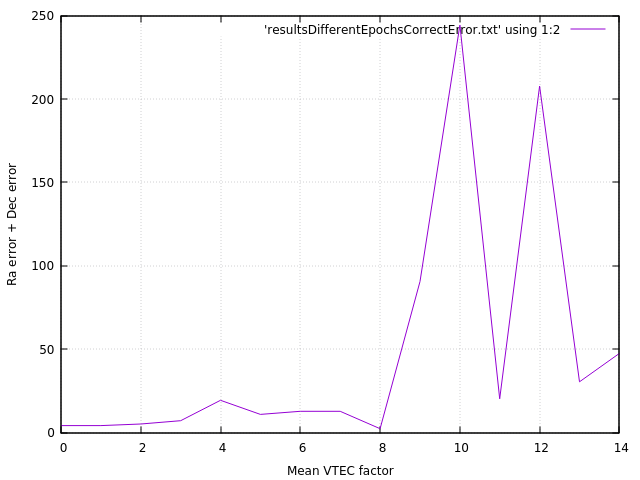
\includegraphics[width=\linewidth]{images/ch6/spikes/decreaseRangeError.png}
		\caption{Error of the estimated source}
	\end{subfigure}
	\caption{Correlation and error of the solution as the mean VTEC decreases}
	\label{fig:differentEpochs}
\end{figure}

As we can see, the correlation rapidly decreases from 1 (almost linear) to a negative coefficient. The error, on the other hand, doesn't experience much change for the first epochs but finally increases considerably. 

The fact that the error remains near 0 as the correlation rapidly decreases for the first epochs can be due to the fact that different location of the source reduces its effect on the  the estimated location with the highest correlation coefficient is still similar to that of the source. As the position of the source changes (the Sun in this case)  TODO: este parrafo

\subsection{Correlation}

As seen in the previous chapter, there exists a correlation between the VTEC value and the cosine of the solar-zenith angle. 

Once the moment of the flare is found, the aim of the algorithm is to study the correlation for each of the possible Suns and yield a fitness indicator for them. 

The main idea for the algorithm is that the higher the correlation, the more accurate the estimated location should be, compared to the real one of the Sun. 

The results will be discussed in the last section of this chapter to see if the previous expectations are true.

\paragraph{Computation}

The correlation between two independent variables is defined as follows:

\begin{equation} \label{eq:coefficient}
r_{xy} = \frac{\sum(x_{i} - \bar{x})(y_{i} - \bar{y})}
{\sqrt{\sum(x_{i} - \bar{x})^{2}}
	\sqrt{\sum(y_{i} - \bar{y})^{2}}} \ \ \text{for} \ \ i \in (0, n)
\end{equation} \\

Although optimization is not the aim of this section, the previous formula would require passing the data twice: first to compute the mean of the cosine and VTEC and second to compute the coefficient itself. The formula can also be expressed as follows:

\begin{equation} \label{eq:singlePass}
r_{xy} = \frac{n\sum x_{i}y_{i} - \sum x_{i}\sum y_{i}}
{\sqrt{n\sum x_{i}^{2} - (\sum x_{i})^{2}}
	\sqrt{n\sum y_{i}^{2} - (\sum y_{i})^{2}}}  \ \ \text{for} \ \ i \in (0, n)
\end{equation} \\

With can be implemented with a single pass algorithm, as opposed to the former. Because of this we decided to initially start with this one.

To ensure that the implementation of the previous method in Fortran was correct, we used the R language and its already implemented correlation function to test our results, in the previous section the Fortran implementation is shown. 

\section{Algorithm}

The algorithm works as follows: the spike of VTEC value throughout the day is found by finding the epoch with the maximum mean VTEC of all IPPs for that epoch\footnote{The use of this method for finding the best epoch is discussed in chapter **** }.
The data is then filtered by that epoch (only the info of IPPs for that epoch will be used for the computations) and the algorithm starts considering possible Suns.

There are $360 * 180 = 64800$ possible Sun's. Thus, in order to test the algorithm, the factor \textit{STEP} is used which defines the step between the angles of possible Suns. The smaller the step, the more Suns will be considered. 

For each of these possible Suns, the VTEC value and the cosine of the solar-zenith angle ($\cos \chi$) are computed for every IPP in that epoch, but the $\cos \chi$ is computed using the location of the IPP and the one of the possible Sun. Each of this Suns yields a data set with the aforementioned variables that can be plotted to obtain images such as the one studied at the end of the previous section. This two variables are used for computing the correlation coefficient for every considered Sun.

The following is the pseudocode for the brute force approach of the algorithm. Which returns the Sun that has yielded the highest correlation coefficient.

\begin{algorithm}
	\caption{Brute Force Approach}\label{pseudocodeBruteForce}
	\begin{algorithmic}[1]
		\Procedure{main}{}
		\State $\textit{epoch} \gets \text{findSpikeInData()}$ 
		\State $\text{filterDataByEpoch(\textit{epoch})}$
		\State $bestSun \gets nil$
		\For {$ra = 0;\ ra <= 360;\ ra += STEP$}
		\For {$dec = -90;\ dec <= 90;\ dec += STEP$}
		\State $currentSun \gets computeCorrelationPossibleSun(ra, dec)$
		\If {$currentSun.correlation > bestSun.correlation$} 
		\State $bestSun \gets currentSun$
		\EndIf
		\EndFor
		\EndFor
		\\
		\Return $bestSun$
		\EndProcedure
	\end{algorithmic}
\end{algorithm}

\clearpage

One thing that has to be taken into consideration is that all possible locations that have a declination of 90º or -90º yield the same results (figure \ref{fig:poles}).

\begin{figure}[!htb]
	\begin{subfigure}[b]{0.5\textwidth}
		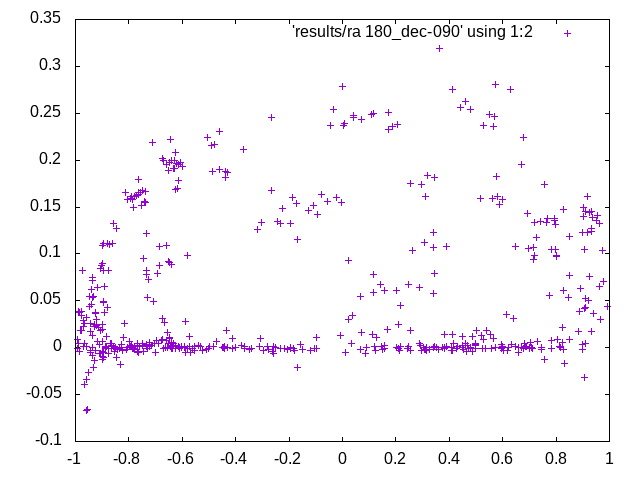
\includegraphics[width=\linewidth]{images/ch4/ra180_dec-090.png}
		\caption{ra=180º, dec=-90º}
	\end{subfigure}
	\hfill
	\begin{subfigure}[b]{0.5\textwidth}
		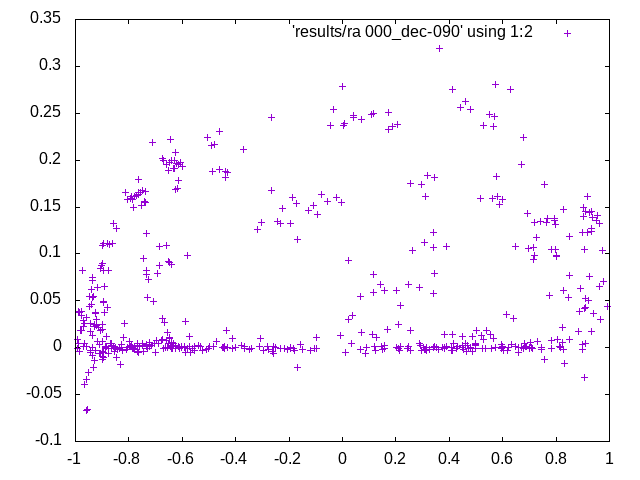
\includegraphics[width=\linewidth]{images/ch4/ra000_dec-090.png}
		\caption{ra=0º, dec=-90º}
	\end{subfigure}
	\caption{Two examples of possible Sun locations}
	\label{fig:poles}
\end{figure}

Using a \textit{diff} tool we can observe that although the data files used to plot the results \footnote{The data is $cos\chi$ as the X axis and VTEC as the Y axis} have different values, the resulting plots are exactly the same image.

This is due to the fact that declinations 90º and -90º correspond to the poles, when the Sun is directly on top or below the Earth, and therefore all possible right ascensions are exactly the same position.

\subsection{Implementation}

\paragraph{Finding the epoch}

\begin{minipage}{\linewidth}
\begin{lstlisting}[language=c, caption=Finding a VTEC spike]
double epochIn, vtecIn, raIPPIn, latIPPIn;
int n = 0;

data >> epochIn >> vtecIn >> raIPPIn >> latIPPIn;
double totalEpochVTEC = vtecIn;
double previousEpoch = epochIn;
while (data >> epochIn >> vtecIn >> raIPPIn >> latIPPIn) {
	totalEpochVTEC += vtecIn;
	n++;
	if (previousEpoch != epochIn) {
		insertCandidate(previousEpoch, totalEpochVTEC/n);
		previousEpoch = epochIn;
		totalEpochVTEC = 0;
		n = 0;
	}
}
\end{lstlisting}
\end{minipage}

The loop traverses the data and computes the mean VTEC of each epoch, inserting it in a priority queue.

\paragraph{Iterating over the possible Suns}
\begin{minipage}{\linewidth}
\begin{lstlisting}[language=c, caption=Main loops]
for (int dec = -90; dec <= 90; dec += step) {
	if (dec != -90 and dec != 90) {
		for (int ra = 0; ra <= 360; ra += step) {
			pearsonCoefficient = computeCorrelation(&ra, &dec);
			if (pearsonCoefficient > maxCoefficient) {
				maxCoefficient = pearsonCoefficient;
				location = "[" + to_string(ra) + ", " + to_string(dec) + "]";
			}
		}
	}
	else {
		int ra = 0;
		pearsonCoefficient = computeCorrelation(&ra, &dec);
		if (pearsonCoefficient > maxCoefficient) {
			maxCoefficient = pearsonCoefficient;
			location = "[" + to_string(ra) + ", " + to_string(dec) + "]";
		}
	}
}
\end{lstlisting}
\end{minipage}

\paragraph{Computing the correlation}

This is the main code of the Fortran function \textit{computeCorrelation(ra, dec)} called for every possible \textit{(ra, dec)} pair (a "virtual" Sun) considered in the previous loop. \textit{computeCorrelation} has more auxiliary functions such as \textit{openFile()} that are not included for readability.

It reads every line of the file that contains the information of the IPPs filtered by the found epoch and computes both the solar-zenith angle and the VTEC as seen in the previous chapter.

Given these results, the necessary values for computing the correlation are updated each iteration:

\begin{itemize}
	\item $\sum x_{i}$ and $\sum y_{i}$
	\item $\sum x_{i}y_{i}$
	\item $\sum x_{i}^{2}$ and $\sum y_{i}^{2}$
\end{itemize}


Once all the IPPs have been processed, the previous values are used to compute the Pearson Correlation Coefficient using equation \ref{eq:singlePass}.

\begin{lstlisting}[language=Fortran, caption=Correlation computation]
double precision function traverseFile (raSunIn, decSunIn)
	implicit none
	integer, intent(in) :: raSunIn, decSunIn
	double precision :: raIPP, decIPP, raSun, decSun, mapIon, d2Li, cosX, vtec
	double precision :: sumx = 0, sumy = 0, sumxy = 0, sumx2 = 0, sumy2 = 0
	double precision :: rxyPearson
	integer :: i = 0
	
	sumx = 0
	sumy = 0
	sumxy = 0
	sumx2 = 0
	sumy2 = 0
	i = 0
	
	raSun = raSunIn
	decSun = decSunIn
	raSun = toRadian(raSun)
	decSun = toRadian(decSun)
	call openFile()
	do while (1 == 1)
		read (1, *, end = 240) raIPP, decIPP, mapIon, d2Li
		raIPP = toRadian(raIPP)
		decIPP = toRadian(decIPP)
		vtec = estimateVTEC(mapIon, d2Li)
		cosx = computeSolarZenithAngle (raIPP, decIPP, raSun, decSun)
		if (cosx > CORRELATION_THRESHOLD) then
			write(34,*) cosx, vtec
			call updateCorrelationParameters (cosx, vtec, sumx, sumy, sumxy, sumx2, sumy2)
			i = i + 1
		end if	
	end do
	240 continue
	close(1)
	rxyPearson = computePearsonCoefficient(i, sumx, sumy, sumxy, sumx2, sumy2)
	return
end function traverseFile
\end{lstlisting}

As can be seen in the code, the line (IPP) is only considered if $\cos\chi$ is higher than a \textit{"correlation threshold"} (-0.1º in this case). This is done because we want to study only the "part" of the ionosphere where the Sun is having an effect. This can be seen in figure \ref{fig:solar-zenith-angle}, where we observed that the VTEC value remained the same from $\cos\chi = -1$ (180º) to $\cos\chi = 1$ (0º).

\paragraph{Compiling}

The C++ and Fortran compilers allow us to compile both languages and their libraries together. With this, the main part of the algorithm can be implemented using C++ which can then call Fortran for the parts that require heavy numerical computation.

This can be done by compiling the object of the Fortran code using the $-c$ flag, and then linking it with the C++ code using the $-lgfortran$ flag so that the standard Fortran libraries are included: \\

\textit{gfortran fortranFunctions.f90 -c -o functions.o}
	
\textit{g++ functions.o bruteForce.cc -o bruteForce.x -lgfortran}

\subsection{Results}

Executing the algorithm with a STEP of 10º, this is the output of the execution:

\begin{lstlisting}[caption=Brute force approach algorithm output]
[C++: Finding a spike in the VTEC distribution]
	-> Spike found: 11.05
[AWK: Filtering all data by best epoch: 11.05]
[C++ -> Fortran: Finding the Person coefficients for possible Suns]
	-> Input degree step: 10
[631 possible Suns considered]
[C++: Results]
	-> Largest correlation coefficient: 0.926959
	-> Estimated Sun's location: [ra=210, dec=-10]
\end{lstlisting}

As we can see, the possible Sun with the highest correlation coefficient (0.9269) has a location with a right ascension of 210º and a declination of -10º. Considering that for the epoch we are working with the Sun position was $212.338º$ and $-13.060º$ as the right ascension and declination, respectively, we can see that the estimated Sun's location returned by the algorithm is close to the real one, using a step of 10º.

It can be interesting to see how the computation time grows as more precision is demanded from the algorithm, and if the precision of the results does as well. The following table shows this relation for some input cases:

\begin{table}[h!]
	\centering
	\def\arraystretch{1.2}
	\begin{tabular}{|c c c c c|} 
		\hline
		Step & Considered Suns & Correlation coefficient & Estimated location & Execution time \\ [0.5ex] 
		\hline\hline
		100 & 5 & 0.695358 & [ra=200, dec=10] & 867ms \\
		\hline 
		50 & 25 & 0.695358 & [ra=200, dec=10] & 303ms \\
			\hline 
		25 & 106 & 0.866293 & [ra=225, dec=-15] & 820ms \\
			\hline 
		12 & 436 & 0.92287 & [ra=216, dec=-6] & 956ms \\
			\hline 
		6 & 1771 & 0.934663 & [ra=216, dec=-12] & 1s 385ms \\
			\hline 
		3 & 7141 & 0.937349 & [ra=213, dec=-12] & 7s 169ms \\
			\hline 
		1 & 64621 & 0.939114 & [ra=214, dec=-11] & 1m 9s 564ms \\
		\hline 
	\end{tabular}
	\caption{Results}
\end{table}

As we can see this approach provides the expected results, but has a large computational complexity that increases with the precision we demand. 

Furthermore, we can see that a problem appears: in the last two cases there is an increase in the correlation coefficient as expected, but the estimated Sun location does not improve, it is actually less accurate than the previous one.

In the next chapter, the \textit{Blind GNSS Search of Extraterrestrial EUV Sources} (BGSEES) algorithm is presented to perform this computations with several optimizations to reduce its complexity and certain special cases are studied, like the aforementioned one.
